\documentclass{standalone}

\usepackage{tikz}
\usepackage{pgfplots}
\usetikzlibrary{calc}
\pgfplotsset{compat=newest}

\begin{document}
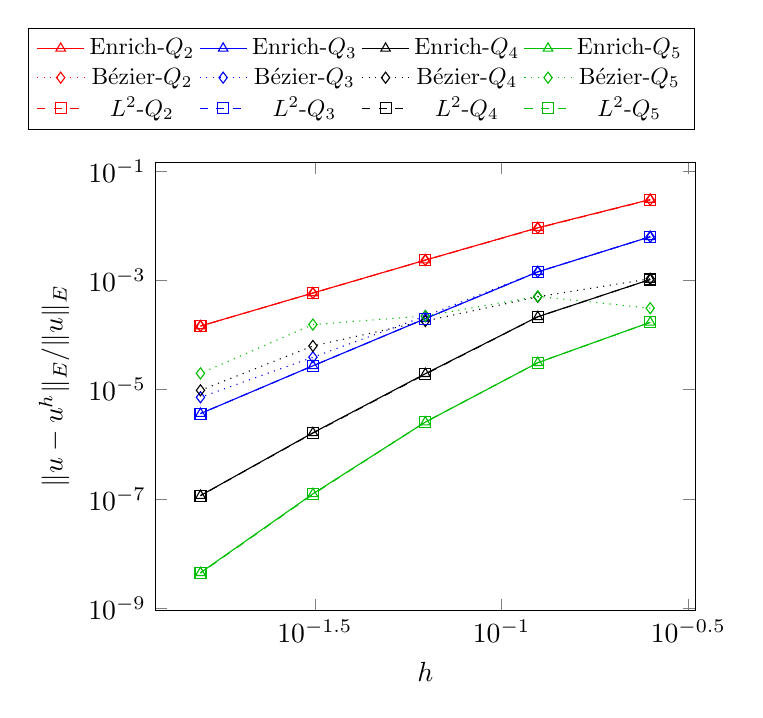
\begin{tikzpicture}
    \begin{loglogaxis}[
        legend columns=4,
    	legend style={at={(1,1.3)}, nodes={scale=.85, transform shape}},
        xlabel=$h$,
        ylabel=${\|u-u^{h}\|_{E}}/{\|u\|_{E}}$ 
    ]

    \addplot [color=red,mark=triangle] plot coordinates {

        (.25,       0.0302658)
        (.125,      0.0092028)
        (.0625,     0.00235437)
        (0.03125,   0.000588624)
        (0.015625,  0.000146344)
    };

    
    \addplot [color=blue,mark=triangle] plot coordinates {

        (.25,       0.00630524)
        (.125,      0.00143356)
        (.0625,     0.000199624)
        (0.03125,   2.73729e-05)
        (0.015625,  3.65571e-06)
    };

    \addplot [color=black,mark=triangle] plot coordinates {

        (.25,       0.00104121)
        (.125,      0.000216016)
        (.0625,     1.96142e-05)
        (0.03125,   1.625e-06)
        (0.015625,  1.15293e-07)
    };

    \addplot [color=green!75!black,mark=triangle] plot coordinates {

        (.25,       0.000171239)
        (.125,      3.12054e-05)
        (.0625,     2.55116e-06)
        (0.03125,   1.24158e-07)
        (0.015625,  4.46807e-09)
    };

    
    \addplot [color=red,mark=diamond, every mark/.append style={solid}, dotted] plot coordinates {

        (.25,       0.0300002)
        (.125,      0.00912921)
        (.0625,     0.00235875)
        (0.03125,   0.000587552)
        (0.015625,  0.000146391)
    };

    
    \addplot [color=blue,mark=diamond, every mark/.append style={solid}, dotted] plot coordinates {

        (.25,       0.00631205)
        (.125,      0.0014356)
        (.0625,     0.000221919)
        (0.03125,   3.92951e-05)
        (0.015625,  7.26411e-06)
    };

    \addplot [color=black,mark=diamond, every mark/.append style={solid}, dotted] plot coordinates {

        (.25,       0.00107166)
        (.125,      0.000502038)
        (.0625,     0.000180486)
        (0.03125,   6.31162e-05)
        (0.015625,  9.74018e-06)
    };

    \addplot [color=green!75!black,mark=diamond, every mark/.append style={solid}, dotted] plot coordinates {

        (.25,       0.000310129)
        (.125,      0.00051043)
        (.0625,     0.000223482)
        (0.03125,   0.000155906)
        (0.015625,  1.9892e-05)
    };


    \addplot [color=red,mark=square, every mark/.append style={solid}, dashed] plot coordinates {

        (.25,       0.0299481)
        (.125,      0.00911375)
        (.0625,     0.00235479)
        (0.03125,   0.00058655)
        (0.015625,  0.000146111)
    };

    
    \addplot [color=blue,mark=square, every mark/.append style={solid}, dashed] plot coordinates {

        (.25,       0.00629887)
        (.125,      0.00143511)
        (.0625,     0.000199702)
        (0.03125,   2.73336e-05)
        (0.015625,  3.65159e-06)
    };

    \addplot [color=black,mark=square, every mark/.append style={solid}, dashed] plot coordinates {

        (.25,       0.00104062)
        (.125,      0.000216071)
        (.0625,     1.91955e-05)
        (0.03125,   1.60067e-06)
        (0.015625,  1.14836e-07)
    };

    \addplot [color=green!75!black,mark=square, every mark/.append style={solid}, dashed] plot coordinates {

        (.25,       0.000171053)
        (.125,      3.11536e-05)
        (.0625,     2.55952e-06)
        (0.03125,   1.21558e-07)
        (0.015625,  4.38487e-09)
    };

    \logLogSlopeTriangle{0.16}{0.075}{0.06}{4.8}{green!75!black};
    \logLogSlopeTriangle{0.16}{0.075}{0.23}{3.8}{black};
    \logLogSlopeTriangle{0.16}{0.075}{0.42}{2.9}{blue};
    \logLogSlopeTriangle{0.16}{0.075}{0.62}{2}{red};

    \legend{Enrich-$Q_2$\\Enrich-$Q_3$\\Enrich-$Q_4$\\Enrich-$Q_5$\\B\'ezier-$Q_2$\\B\'ezier-$Q_3$\\B\'ezier-$Q_4$\\B\'ezier-$Q_5$\\$L^2$-$Q_2$\\$L^2$-$Q_3$\\$L^2$-$Q_4$\\$L^2$-$Q_5$\\}
    \end{loglogaxis}
\end{tikzpicture}

\end{document}
